\section{Results}
% prec:0.154787009701     f1:0.179024390244       jac:0.0983123493169

We performed experiments to evaluate the performance of the feature classification. The experimental setup described in the previous section shows that we have many parameters that could influence the classification performance. We will therefore first show results for a certain set of parameters that performed well. In the further sections, we explore the effects of different parameters, such as different feature parameters, classification algorithms, and test images.

%In this case, the classifiers were trained on section two and three and tested on section one. Furthermore, these results were obtained using synthetic oversampling using the SMOTE method.


\begin{figure}
	\centering
	\begin{tabular}{cc}
		\subfloat{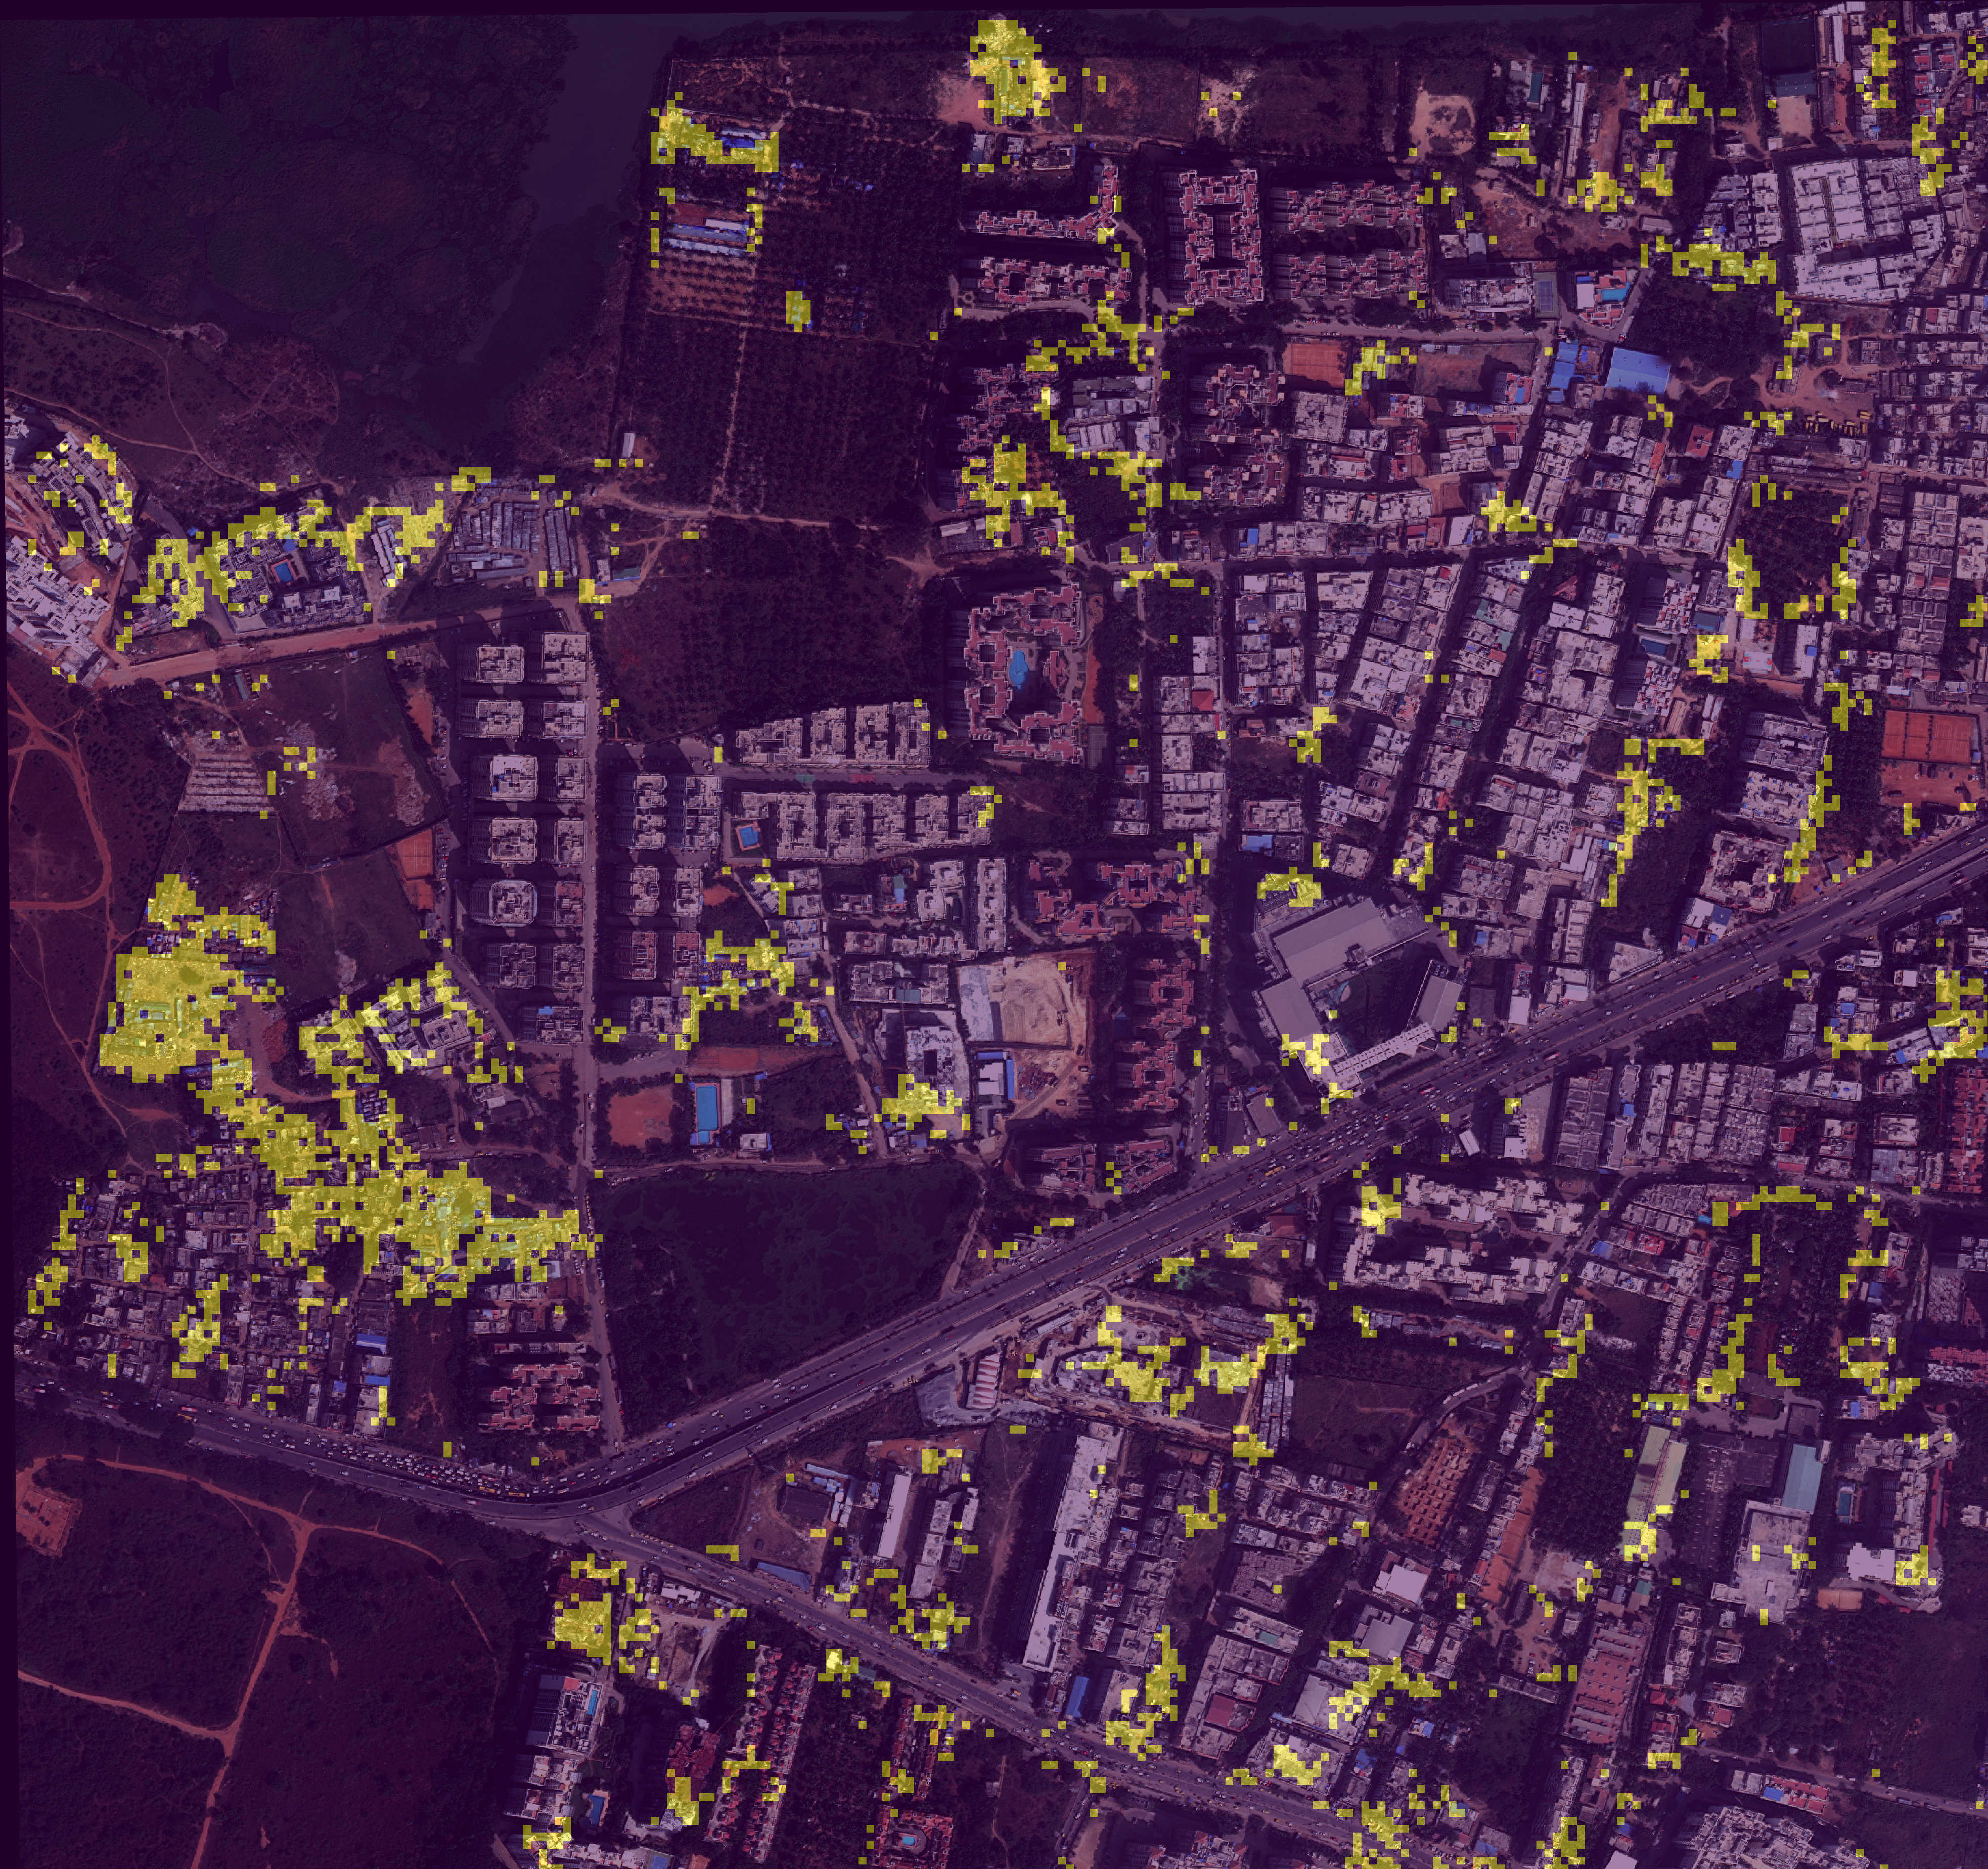
\includegraphics[width=7cm]{images/BestOverlay}}&
		\subfloat{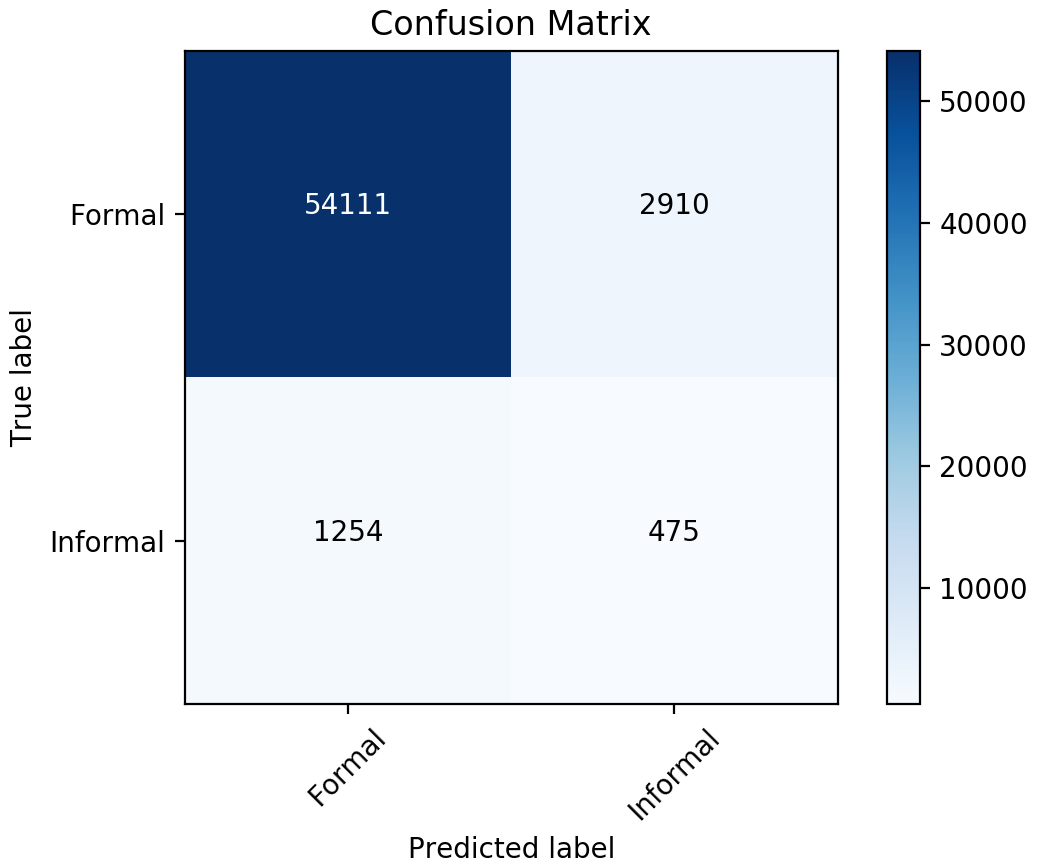
\includegraphics[height=7cm]{images/BestConfusion}}
	\end{tabular}
	\caption{Classification of Section 2 using Gradient Boosting}
	\label{fig:res_best}
\end{figure}

Figure \ref{fig:res_best} shows the most fitting classification we could achieve using our current features and classifiers. The results are produced by the experiment described in the experimental setup. For this specific classifcation, we used the second section using all three features, the scales 50, 100 and 150 and Gradient Boosting. It achieved a F1-Score of 0.179 and a Jaccard's index of 0.098. The confusion matrix in the same figure displays the number of correct and incorrect classifications.

\subsection{Feature Performance}

\pgfplotstableread[col sep = comma]{results/features_sections.csv}\datazero

\begin{figure}
	\begin{tikzpicture}
	\begin{axis}[
	ybar,
	ymajorgrids = true,
	bar width=0.5cm,
	ylabel = Matthews Coefficient,
	width=\textwidth,
	height=.5\textwidth,
	enlarge x limits=0.25,
	symbolic x coords={Section 1, Section 2, Section 3},
	xtick=data,
	yticklabel style={
		/pgf/number format/fixed,
		/pgf/number format/precision=2,
		/pgf/number format/fixed zerofill
	},
	scaled y ticks=false,
	legend columns=4, 
	legend style={
		% the /tikz/ prefix is necessary here...
		% otherwise, it might end-up with `/pgfplots/column 2`
		% which is not what we want. compare pgfmanual.pdf
		/tikz/column 2/.style={
			column sep=5pt,
		},
		at={(0.75, -0.15)},
	}
	]
	\addplot table[x=TestImage, y=HoG]{\datazero};
	\addplot table[x=TestImage, y=LSR]{\datazero};
	\addplot table[x=TestImage, y=RID]{\datazero};
	\addplot table[x=TestImage, y=All features]{\datazero};
	%\addplot[dotted, sharp plot, update limits=false] coordinates {(0, 0)(1, 0)}; 
	\legend{HoG, LSR, RID, All features}
	\end{axis}
	
	\end{tikzpicture}
	\caption{The performance of features}
	\label{fig:res_bar_0}
\end{figure}

The bar plot in Figure \ref{fig:res_bar_0} show the classification performance for the four feature sets on the three sections. To save space, we only display the results of the classifier with the highest performance.
It seems that HoG performs well for all three sections. LSR is more variable between the three sections. In the second section, LSR is close to HoG in performance, but in section three, it really underperforms. RID seems reasoanble in the first section, but it fails for the other two sections. The combined features seems to perform well, although not better than HoG alone in any section.


\subsection{Classifier Performance}

Although Figure \ref{fig:res_bar_0} shows the maximum performance of the features, it does not display the individual performance of the classifiers. We therefore compare the classification algorithms side by side to gain more insight in the performance differences of the classification algorithms. This comparison is displayed in Figure \ref{fig:res_bar_1}. The bar plot displays the maximum performance that a classifier has obtained for any feature set or test image. Because we measure performance using two different metrics, we chose the maximum of both metrics. As a side note: we discovered that, for all classifiers, the set of parameters that produced the maximum of Matthews Coefficient was the same set of parameters with the maximum F1-score. That the measurements by two different algorithms is similar suggests that the measure of performance is consistent.

\pgfplotstableread[col sep = comma]{results/classifiers.csv}\dataone

\begin{figure}
	\begin{tikzpicture}
		\begin{axis}[
			ybar,
			bar width=.5cm,
			width=\textwidth,
			height=.5\textwidth,
			legend pos = north west,
			ylabel= Maximum Performance,
			symbolic x coords={DecisionTree, RandomForrest,AdaBoost,GradientBoost,MLP},
			xtick=data,
			yticklabel style={
				/pgf/number format/fixed,
				/pgf/number format/precision=2,
				/pgf/number format/fixed zerofill
			},
			scaled y ticks=false,
		]
		\addplot table[x=Classifier,y=F1-Score]{\dataone};
		\addplot table[x=Classifier,y=Matthews]{\dataone};
	
	
		\legend{F1-Score, Matthews Coefficient}
		\end{axis}
		
	\end{tikzpicture}
	\caption{Maximum Performance of the Classification Algorithms for all sections}
	\label{fig:res_bar_1}
\end{figure}

Figure \ref{fig:res_bar_1} shows that Gradient Boosting was able to produce the best results. However, note that this is only the maximum performance for a certain set of parameters. It does not necessarily follow that this level of performance is also achieved for different parameters.
% TODO: verder?

\subsection{Effect of different Scales}

As we have shown in the feature evaluation, we suspect increased scale to have a positive effect on the classification performance of the features. In this experiment, the only variable is the different scales. The all other parameters are fixed. We use a single feature set containing all features and section 1 as the test image. We use Matthews coefficient to display the difference in performance.

%\pgfplotstableread[row sep=\\,col sep=&]{
%	Scale	 & Precision & F1-Score	& Jaccard \\
%	50		 & 0.088764742396027 & 0.1505923650724 	 & 0.081427351238493\\
%	100 	 & 0.130880333759995 & 0.198156164860832 & 0.109974106030222\\
%	150		 & 0.12144780137601  & 0.160094637223975 & 0.087012430347193\\
%	All three & 0.158875401704021 & 0.184835731052331 & 0.101828652373582\\
%}\datathree
%
%\begin{figure}
%	\begin{tikzpicture}
%	\begin{axis}[
%	ybar,
%	bar width=.5cm,
%	width=\textwidth,
%	height=.5\textwidth,
%	symbolic x coords={50, 100, 150, All three},
%	xtick=data,
%	yticklabel style={
%		/pgf/number format/fixed,
%		/pgf/number format/precision=2,
%		/pgf/number format/fixed zerofill
%	},
%	scaled y ticks=false,
%	legend pos=north west,
%	]
%	\addplot table[x=Scale,y=Precision]{\datathree};
%	\addplot table[x=Scale,y=F1-Score]{\datathree};
%	\addplot table[x=Scale,y=Jaccard]{\datathree};
%	\legend{Precision, F1-Score, Jaccard's Index}
%	\end{axis}
%	
%	\end{tikzpicture}
%	\caption{Performance for different scales}
%	\label{fig:res_bar_3}
%\end{figure}


\begin{figure}
	\centering
	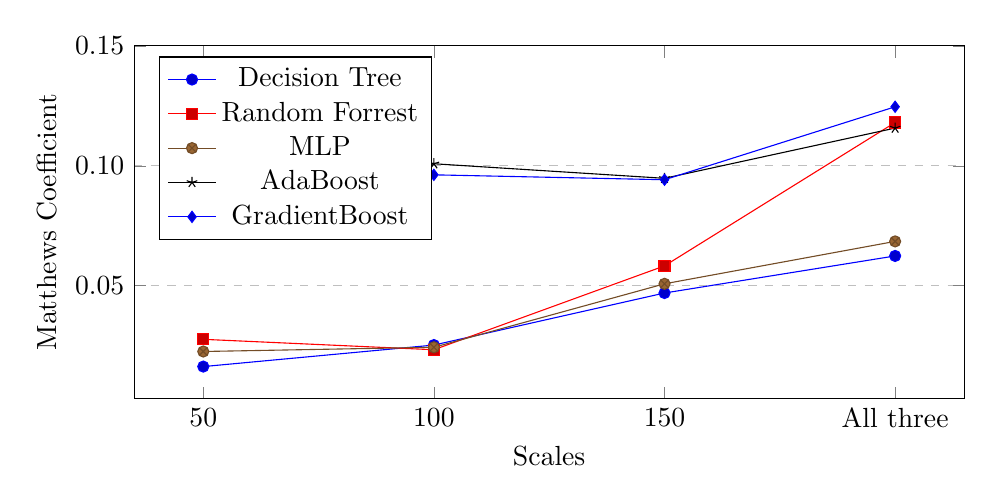
\begin{tikzpicture}
	\begin{axis}[
		title={},
		xlabel={Scales},
		ylabel={Matthews Coefficient},
		width=\textwidth,
		height=.5\textwidth,
		symbolic x coords={50, 100, 150, All three},
		xtick=data,
		ytick={0.0, 0.05, 0.10, 0.15},
		yticklabel style={
					/pgf/number format/fixed,
					/pgf/number format/precision=2,
					/pgf/number format/fixed zerofill
				},
		ymax=0.15,
		legend pos=north west,
		ymajorgrids=true,
		grid style=dashed,
		]
	
		\addplot
		coordinates {
			(50, 0.016316391931366)(100, 0.025284087065911)(150, 0.046978019893256)(All three, 0.062425136350308)
		};
		
		\addplot
		coordinates {
			(50, 0.02767643490798)(100, 0.023335494910068)(150, 0.058283285951452)(All three, 0.118049918431825)
		};
		
		\addplot
		coordinates {
			(50,0.022601460220282 )(100, 0.024361604826938)(150, 0.05081177009644)(All three, 0.068491183148441)
		};
		\addplot
		coordinates {
			(50, 0.075135546760044)(100,0.10084290115786 )(150, 0.094779745284877)(All three, 0.115714829966404)
		};
		\addplot
		coordinates {
			(50, 0.073269806673298 )(100, 0.096228849171068)(150, 0.094189254108157)(All three, 
			0.124593317547984)
		};
		\legend{Decision Tree, Random Forrest, MLP, AdaBoost, GradientBoost}
		
	
	\end{axis}
	\end{tikzpicture}
	\caption{Effects of increased scale for all features on section 1 as test image}
	\label{fig:res_plot_0}
\end{figure}

After observing Figure \ref{fig:res_plot_0}, it seems that increased scale, or at least a combination of scales results in improves classification performance. To test the generizability, we ran the same experiment with section 2 as test image, and we observed that this did not necessarily produce the same result. For section 2, the highest performance is achieved for the combination of all features, followed by scale 50. The performance actually regesses from scale 50 to scale 150 before increasing again with the combination of all features. This leads us to conclude that we are indecisive if increased scale improves performance in general. It might be depended on the data used.

%\subsection{Effects of oversampling}
%As hinted earlier, oversampling is an important part in classification. Without oversampling, the classifiers are likely to produce trivial results. Oversampling is a common method to balance a dataset. In this section, we evaluate three different oversampling methods. These are random oversampling, SMOTE and ADASYN. The first method randomly picks entries of the minority class and copies these. The last two methods create new synthetic examples that suit the data well.
%%TODO: extend


